% Two-column article layout keeps this source portable to local TeX and Overleaf.
\documentclass[twocolumn,10pt]{article}
\usepackage[margin=0.72in,columnsep=0.25in]{geometry}
\usepackage{graphicx}
% Local pdflatex runs from this directory; Overleaf runs from the project root.
\graphicspath{{../../results/plots/}{results/plots/}}
\usepackage{amsmath}
\usepackage{booktabs}
\usepackage{url}
\usepackage{array}
\usepackage[T1]{fontenc}
\usepackage{lmodern}
\ifdefined\pdfgentounicode
  \input{glyphtounicode}
  \pdfgentounicode=1
\fi
\title{Look-Ahead Handoffs and Runtime-Adaptive Bank Eligibility\\for a Tiled Neural-Network Scratchpad}
\author{Jayesh Motwani\textsuperscript{1}, Kia Wadher\textsuperscript{2},
and Vedansh Belwal\textsuperscript{3}\\
School of Electronics Engineering, VIT Vellore\\[0.25em]
{\small \textsuperscript{1}\texttt{jayesh.motwani2024@vitstudent.ac.in}}\\
{\small \textsuperscript{2}\texttt{kia.chetanwadher2024@vitstudent.ac.in}}\\
{\small \textsuperscript{3}\texttt{vedansh.belwal2024@vitstudent.ac.in}}}
\date{}
\begin{document}
\maketitle
\begin{abstract}
Scratchpad buffering and controller handoff timing can independently limit
a neural-network accelerator's multiply-accumulate (MAC) utilization. We
implement runtime bank eligibility and completion-aware look-ahead handoffs
in one Verilog design with four physical RAM banks, one loader, and one MAC.
The depth policy uses a 32-cycle starvation window and integer 8/2
hysteresis thresholds to permit new allocations to two, three, or four
banks while allowing existing tiles to drain. The handoff scheduler accepts
a new load or MAC descriptor on the edge that the previous operation
finishes; per-tile transfer and compute service times remain unchanged.
Self-checking RTL simulations validate arithmetic results, bank ownership,
and per-tile service intervals under stable, variable-latency, and
phase-changing workloads. For 64 balanced
tiles, adaptive look-ahead execution requires 522 cycles compared with 713
for fixed four-bank allocation with registered handoffs, a 26.79\%
reduction. Variable and phase-changing
workloads take 925 versus 983 and 1808 versus 1991 cycles, reductions of
5.90\% and 9.19\%. The corresponding average allocation limits are 2.061,
3.069, and 2.619 banks. The proposed controller combines handoff scheduling
and eligibility control while retaining the same four physical RAM banks,
one loader, and one MAC. The measurements characterize execution cycles
and allocation eligibility; clock frequency, SRAM power, and physical area
are not measured.
\end{abstract}
\noindent\textbf{Index Terms---} neural-network accelerator, scratchpad,
bank allocation, look-ahead scheduling, Verilog RTL, adaptive control.

\section{Introduction}
Data movement and reuse often dominate accelerator design decisions
\cite{sze2017survey}. A scratchpad keeps a tile near the MAC, and ping-pong
buffering can load tile $t+1$ while tile $t$ is computed. Two banks,
however, hold only two independent tiles. A third or fourth bank can help
when the transfer stream is irregular; when computation is consistently
slower, those extra eligible slots may provide no cycle benefit. A fixed
four-bank policy cannot distinguish these regimes.

Buffer capacity alone does not determine utilization. Registered control
interfaces can introduce idle cycles between successive operations even
when a tile is available. This study evaluates bank eligibility and handoff
timing as independent control dimensions within a four-bank scratchpad.
Runtime eligibility restricts load allocations to two, three, or four
banks, while completion-aware handoffs permit a resource to accept its next
descriptor on the edge that its current operation finishes. Tile values,
RAM timing, input order, and the single-loader, single-MAC organization
are held constant.

The contributions are: (1) a runtime bank-allocation rule with explicit
ownership invariants and safe draining during depth reduction; (2) loader
and MAC handoff logic that eliminates control gaps without shortening
per-tile service intervals; and (3) a controlled RTL evaluation against
single buffering, ping-pong, and fixed four-bank allocation. The primary
baseline, Fixed 4, uses four eligible banks and registered resource
handoffs. The Proposed controller combines adaptive two/three/four-bank
eligibility with completion-aware handoffs. Both use the same RAM and MAC
organization. RH and LH denote registered and look-ahead handoffs when
describing their control timing.

\section{Background and Related Work}
The survey by Sze \emph{et al.} relates arithmetic reuse to movement among
the memory hierarchy levels \cite{sze2017survey}. Eyeriss demonstrates
distributed local storage and row-stationary data reuse
\cite{chen2017eyeriss}. The datacenter TPU uses a software-managed on-chip
memory in a complete inference system \cite{jouppi2017tpu}. Eyeriss v2
adds flexibility for layer shapes and sparsity \cite{chen2019eyerissv2}.
These systems justify careful treatment of on-chip storage, but their
frame rates and full-system speedups cannot be compared directly with our
single-MAC tile-cycle model.

At the controller level, single buffering serializes transfer and compute.
Ping-pong permits overlap but can block the loader while one bank is
computing and the other is occupied. A fixed deeper buffer offers more tile
slots. Runtime eligibility adjusts the allocation limit in response to
compute starvation, whereas look-ahead scheduling reduces the control
latency between resource assignments. The static cyclic policy provides
a fixed tile-to-bank mapping against which availability arbitration can be
evaluated at equal bank count. Table~\ref{tab:prior} summarizes the scope
and evaluation metrics of the related accelerator designs.

\begin{table*}[t]
\centering\caption{Storage and control scope of related accelerator designs.
Published performance values refer to their respective workloads and
platforms; they do not form a common numerical comparison.}
\label{tab:prior}\small
\setlength{\tabcolsep}{4pt}
\begin{tabular}{>{\raggedright\arraybackslash}p{.13\textwidth}>{\raggedright\arraybackslash}p{.30\textwidth}>{\raggedright\arraybackslash}p{.29\textwidth}>{\raggedright\arraybackslash}p{.17\textwidth}}
\toprule
Work & Main storage/control scope & Reported evidence & Relation to this paper\\
\midrule
Eyeriss \cite{chen2017eyeriss} & Distributed local storage and
row-stationary reuse in a CNN chip & AlexNet convolution, batch 4:
35 frames/s and 0.0029 DRAM accesses/MAC & Motivates local reuse;
different hardware and metric\\
TPU \cite{jouppi2017tpu} & Software-managed on-chip memory feeding an
inference systolic array & Production inference: roughly 15--30$\times$
over contemporary CPU/GPU systems & Full-system context only\\
Eyeriss v2 \cite{chen2019eyerissv2} & Flexible hierarchy for varied and
sparse DNN layers & Sparse MobileNet, batch 1: 1470.6 inferences/s and
12.6$\times$ original Eyeriss & Flexibility context only\\
\textbf{This work} & Four-bank tile scratchpad with runtime depth and
look-ahead handoffs & Matched RTL cycles, service traces,
and average eligibility & Direct comparison with internal baselines\\
\bottomrule
\end{tabular}
\end{table*}

\section{Architecture and RTL Implementation}
\subsection{Common Data Path and Bank Protocol}
Figure~\ref{fig:arch} shows the implemented structure. Each tile contains
$T$ activation-weight pairs of width $W$ per operand. A single loader
writes one pair per active clock into a synchronous RAM bank. A read mux
feeds one MAC, which reads one pair per clock and accumulates $T$ products.
The transfer target specifies the effective tile-load interval; the compute
target may include latency after useful MAC operations. Four physical banks remain present in the
runtime design. Bank-depth policies change the choice of a bank for the next
tile. Handoff scheduling determines when the loader and MAC can accept
their next descriptors.

\begin{figure*}[t]
\centering
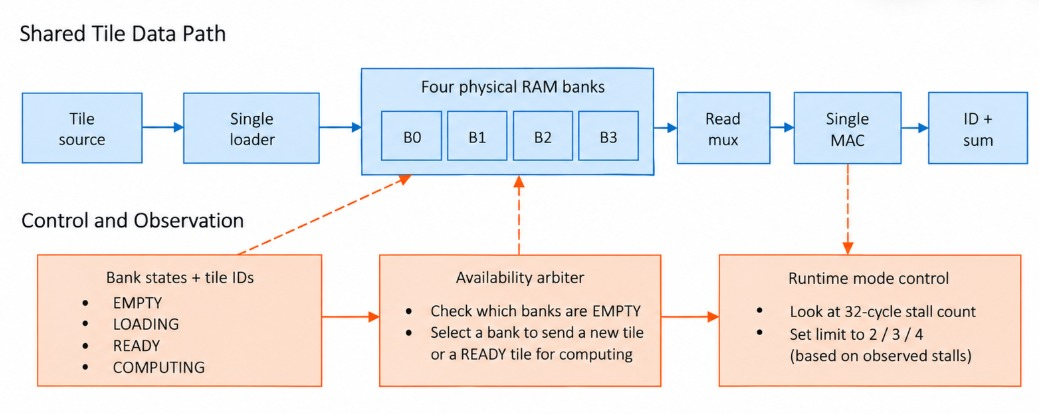
\includegraphics[width=.86\textwidth]{paper_architecture.jpg}
\caption{Implemented data path and runtime control. One loader and one MAC
are shared across four physical RAM banks. The mode controller changes only
which EMPTY banks may receive new tiles; the arbiter may still dispatch a
READY tile from any bank. Blue arrows carry data; orange arrows carry
control or feedback.}
\label{fig:arch}
\end{figure*}

The per-bank protocol in Fig.~\ref{fig:bankfsm} has states EMPTY, LOADING,
READY, and COMPUTING. The loader may claim only an EMPTY bank. Finishing the
programmed load interval makes that bank READY. The MAC claims a READY bank
and releases it to EMPTY only after the result is registered. Each bank
retains a tile ID, so availability dispatch need not return results in input
order. Under RH control, a freed bank becomes eligible for arbitration on
the following clock. LH control uses completion predicates to permit bank
release and descriptor acceptance on the same edge.

\begin{figure}[t]
\centering
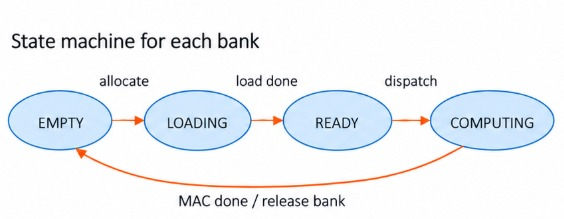
\includegraphics[width=.96\columnwidth]{paper_bank_state_machine.jpg}
\caption{Logical per-bank state transitions. Look-ahead scheduling can
combine completion and the next acceptance at one edge; an unfinished tile
is never overwritten.}
\label{fig:bankfsm}
\end{figure}

\begin{table*}[t]
\centering\caption{Controlled policy distinction. All policies use the same
RAM, operands, loader, MAC, and tile stream. ``Limit'' affects only new
load allocations.}
\label{tab:policies}\small
\setlength{\tabcolsep}{2.5pt}
\begin{tabular}{>{\raggedright\arraybackslash}p{.15\textwidth}>{\raggedright\arraybackslash}p{.10\textwidth}>{\raggedright\arraybackslash}p{.28\textwidth}>{\raggedright\arraybackslash}p{.29\textwidth}>{\raggedright\arraybackslash}p{.12\textwidth}}
\toprule
Policy & Banks & Load allocation & Compute dispatch & Limit\\
\midrule
Single & 1 & Fixed bank; wait until EMPTY & Strict tile order & Fixed 1\\
Ping-pong & 2 & Tile ID modulo 2 & Strict tile order & Fixed 2\\
Availability & 4 & Any EMPTY bank, round-robin & Any READY bank, round-robin & Fixed 4\\
Static cyclic proxy & 4 & Tile ID modulo 4 & Strict tile order & Fixed 4\\
Runtime (proposed) & 4 & EMPTY bank below limit, round-robin & Any READY bank, round-robin & 2, 3, or 4\\
\bottomrule
\end{tabular}
\end{table*}

Table~\ref{tab:policies} isolates both bank count and scheduling policy.
Single and ping-pong assign a tile to a fixed bank by its ID and dispatch
strictly in order. The four-bank availability policy searches EMPTY banks
round-robin for loading and READY banks round-robin for computing. The
static cyclic proxy has the same four tile slots but a fixed ID-to-bank
mapping, so it can test whether availability arbitration adds value beyond
capacity. The runtime policy reuses the availability arbiter, but rejects
an EMPTY bank with index at or above the current allocation limit.

\subsection{Runtime Bank-Limit Algorithm}
The proposed limit $B_c\in\{2,3,4\}$ starts at two and applies to new load
allocations. The compute arbiter always searches all four banks. Thus, if
the limit falls from four to three while bank 3 is READY or COMPUTING, its
tile remains valid and can finish. No migration, invalidation, or discarded
partial sum is required. This asymmetry between allocation and dispatch is
the safety condition for a downward transition.

At each measured clock, a narrow starvation event $s_c$ is one when work
remains, the MAC is free, no dispatch is pending, and no bank is READY.
The controller accumulates these events over $L=32$ clocks. The update at
the window boundary uses the just-observed event as well as the stored
count. Figure~\ref{fig:modefsm} and the pseudocode in
Fig.~\ref{alg:mode} state the
entire rule. High and low thresholds are $H=8$ and $D=2$. Counts from
three through seven hold the current mode; limits saturate at two and four.
Only comparisons and a one-step increment or decrement are required in RTL.

\begin{figure}[t]
\centering
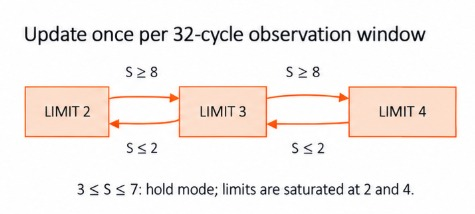
\includegraphics[width=.98\columnwidth]{paper_mode_state_machine.jpg}
\caption{Hysteresis state machine. $S$ is the accumulated no-READY count
over one observation window; each transition changes the allocation limit
by exactly one bank.}
\label{fig:modefsm}
\end{figure}

\begin{figure}[t]
\small
\hrule\vspace{3pt}
\noindent\textbf{Algorithm: Runtime allocation-limit update}\\[2pt]
\noindent\textbf{State:} limit $B\leftarrow 2$, window count $q\leftarrow 0$,
stall count $S\leftarrow 0$.\\
\noindent\textbf{Each measured clock:}\\
\hspace*{1em}Find an EMPTY load bank with index $<B$; dispatch a READY
bank from indices $0$--$3$.\\
\hspace*{1em}$s\leftarrow 1$ iff work remains, MAC is free, no start or
completion is pending, and READY count is zero; else $s\leftarrow 0$.\\
\hspace*{1em}$q\leftarrow q+1$; $S\leftarrow S+s$.\\
\hspace*{1em}\textbf{if} $q=32$ \textbf{then}\\
\hspace*{2em}\textbf{if} $S\geq8$ \textbf{then} $B\leftarrow\min(4,B+1)$;\\
\hspace*{2em}\textbf{else if} $S\leq2$ \textbf{then}
$B\leftarrow\max(2,B-1)$;\\
\hspace*{2em}$q\leftarrow0$; $S\leftarrow0$.\\
\vspace{3pt}\hrule
\caption{Pseudocode of the window update and bank eligibility. The RTL
implements this with nonblocking sequential state updates; the count
includes the event on the closing clock.}
\label{alg:mode}
\end{figure}

\subsection{Completion-Aware Look-Ahead Handoffs}
The RH MAC interface registers a start request and observes a
registered completion, leaving three idle clocks between successive MAC
jobs even when data are queued. The loader similarly leaves one clock
between transfers when another bank is free. A depth restriction alone
cannot remove these costs or add scheduling opportunities beyond fixed
four. The proposed controller removes these gaps by enabling
completion-aware issue in both the loader and the MAC.

With loader look-ahead, the scheduler accepts the next descriptor when the
current transfer reaches its unchanged target, and may reclaim a bank whose
MAC operation completes on that edge. With MAC look-ahead, the next
descriptor is chosen combinationally when the engine is idle or finishing.
Eligible sources are a READY bank or the bank whose load finishes on this
edge. Let $L_f$ and $M_f$ denote these completion predicates. Then the
effective availability conditions are
\begin{align}
E_b^*&=(\operatorname{state}_b=\mathrm{EMPTY})
       \lor(M_f\land b=b_{\rm MAC}),\\
R_b^*&=(\operatorname{state}_b=\mathrm{READY})
       \lor(L_f\land b=b_{\rm load}).
\end{align}
The allocation-limit check still applies to $E_b^*$. The MAC searches all
banks using $R_b^*$, preserving safe drain on a limit decrease.

The MAC asserts $M_f$ only after all $T$ synchronous RAM responses have
been accumulated and its programmed service target has elapsed. On a
chained acceptance edge, nonblocking assignments capture the completed result and
tile ID before resetting the accumulator for the next job. A completing
load can feed a new MAC job safely: the last write occurs on the acceptance
edge, while the first read of the new job occurs on the following edge.
Bank release uses $M_f$, independently of the delayed result notification,
so the notification cannot accidentally free a newly assigned bank.

\begin{figure*}[t]
\centering
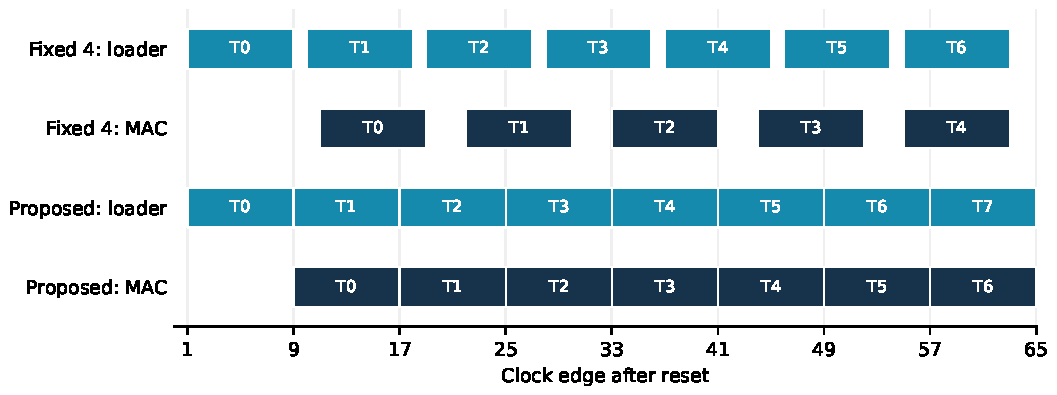
\includegraphics[width=.94\textwidth]{lookahead_handoff_timing.pdf}
\caption{Loader and MAC execution for Fixed 4 and the proposed controller
under the balanced workload. Each interval corresponds to an eight-clock
tile operation. The proposed handoffs eliminate the three-clock MAC gap and
the one-clock loader handoff gap.}
\label{fig:handoff}
\end{figure*}

\subsection{Cycle Accounting and Metrics}
For total measured cycles $C$, active MAC cycles $C_{\rm MAC}$, completed
tiles $N$, and effective limit $B_c$ at clock $c$, we report
\begin{equation}
U=\frac{C_{\rm MAC}}{C},\quad
R=\frac{N}{C},\quad
\bar B=\frac{1}{C}\sum_{c=1}^{C} B_c.
\label{eq:metrics}
\end{equation}
The broad \emph{compute-idle} or \emph{stall} count is $C-C_{\rm MAC}$;
it includes initial fill and handoff, whereas $s_c$ is the narrower signal
that drives adaptation. Speedup equals baseline cycles divided by candidate
cycles. Average limit $\bar B$ measures allocation eligibility, not the
number of physically disabled RAMs; no clock gating or bank power shutoff
is modeled.

\subsection{Control Invariants and Implementation Cost}
With look-ahead disabled, the bank protocol gives two local safety
conditions at every clock $c$:
\begin{align}
\operatorname{allocate}(b,c)&\Rightarrow
  (\operatorname{state}_b=\mathrm{EMPTY})\land(b<B_c),\\
\operatorname{dispatch}(b,c)&\Rightarrow
  \operatorname{state}_b=\mathrm{READY}.
\end{align}
The dispatch condition intentionally has no $b<B_c$ term. It permits a
tile already in a high-index bank to drain after a limit decrease. The RTL
also keeps at most one LOADING and one COMPUTING bank because each resource
has one busy flag and one active-bank register. Result tile IDs let the
testbench check exactly-once completion independently of dispatch order.
With look-ahead enabled, $E_b^*$ and $R_b^*$ replace the state predicates;
the completion edge transfers ownership without overlapping active users.

For four banks, the adaptation state consists of a window counter,
a starvation counter, and the limit register; mode-time and transition
counters are measurement instrumentation. The combinational eligibility
search examines the bounded bank-state array, and the update uses integer
comparisons rather than a division. This describes RTL structure, not
post-synthesis area or critical-path timing.

\subsection{Logic Synthesis}
Yosys 0.69 is used to synthesize the parameterized RTL into generic gate
netlists. Table~\ref{tab:synthesis} compares configurations with four
four-word banks, eight-bit operands, 64 tiles, and fixed 8/8 service targets.
The proposed controller requires 4713 logic/register cells compared with
3477 for Fixed 4, an increase of 35.55\%. Both configurations pass the structural checks without
inferred latches. Cell totals exclude five scope metadata records per
netlist and include the measurement counters and flip-flop RAM mapping.

\begin{table}[t]
\centering\caption{Generic synthesis results under matched hardware and
workload parameters. Register bits are included in the cell totals.}
\label{tab:synthesis}\scriptsize
\begin{tabular}{lrr}
\toprule
Configuration & Logic/register cells & Register bits\\
\midrule
Fixed 4 & 3477 & 595\\
Proposed & 4713 & 864\\
\bottomrule
\end{tabular}
\end{table}

Figure~\ref{fig:gateram} shows the synthesized RAM structure for a
two-word, one-bit instance of the same parameterized RTL. Two enabled
storage elements feed a read multiplexer and a registered output. This
reduced instance exposes the storage and read-path logic; the accelerator
measurements use the wider, deeper banks specified above.

\begin{figure}[t]
\centering
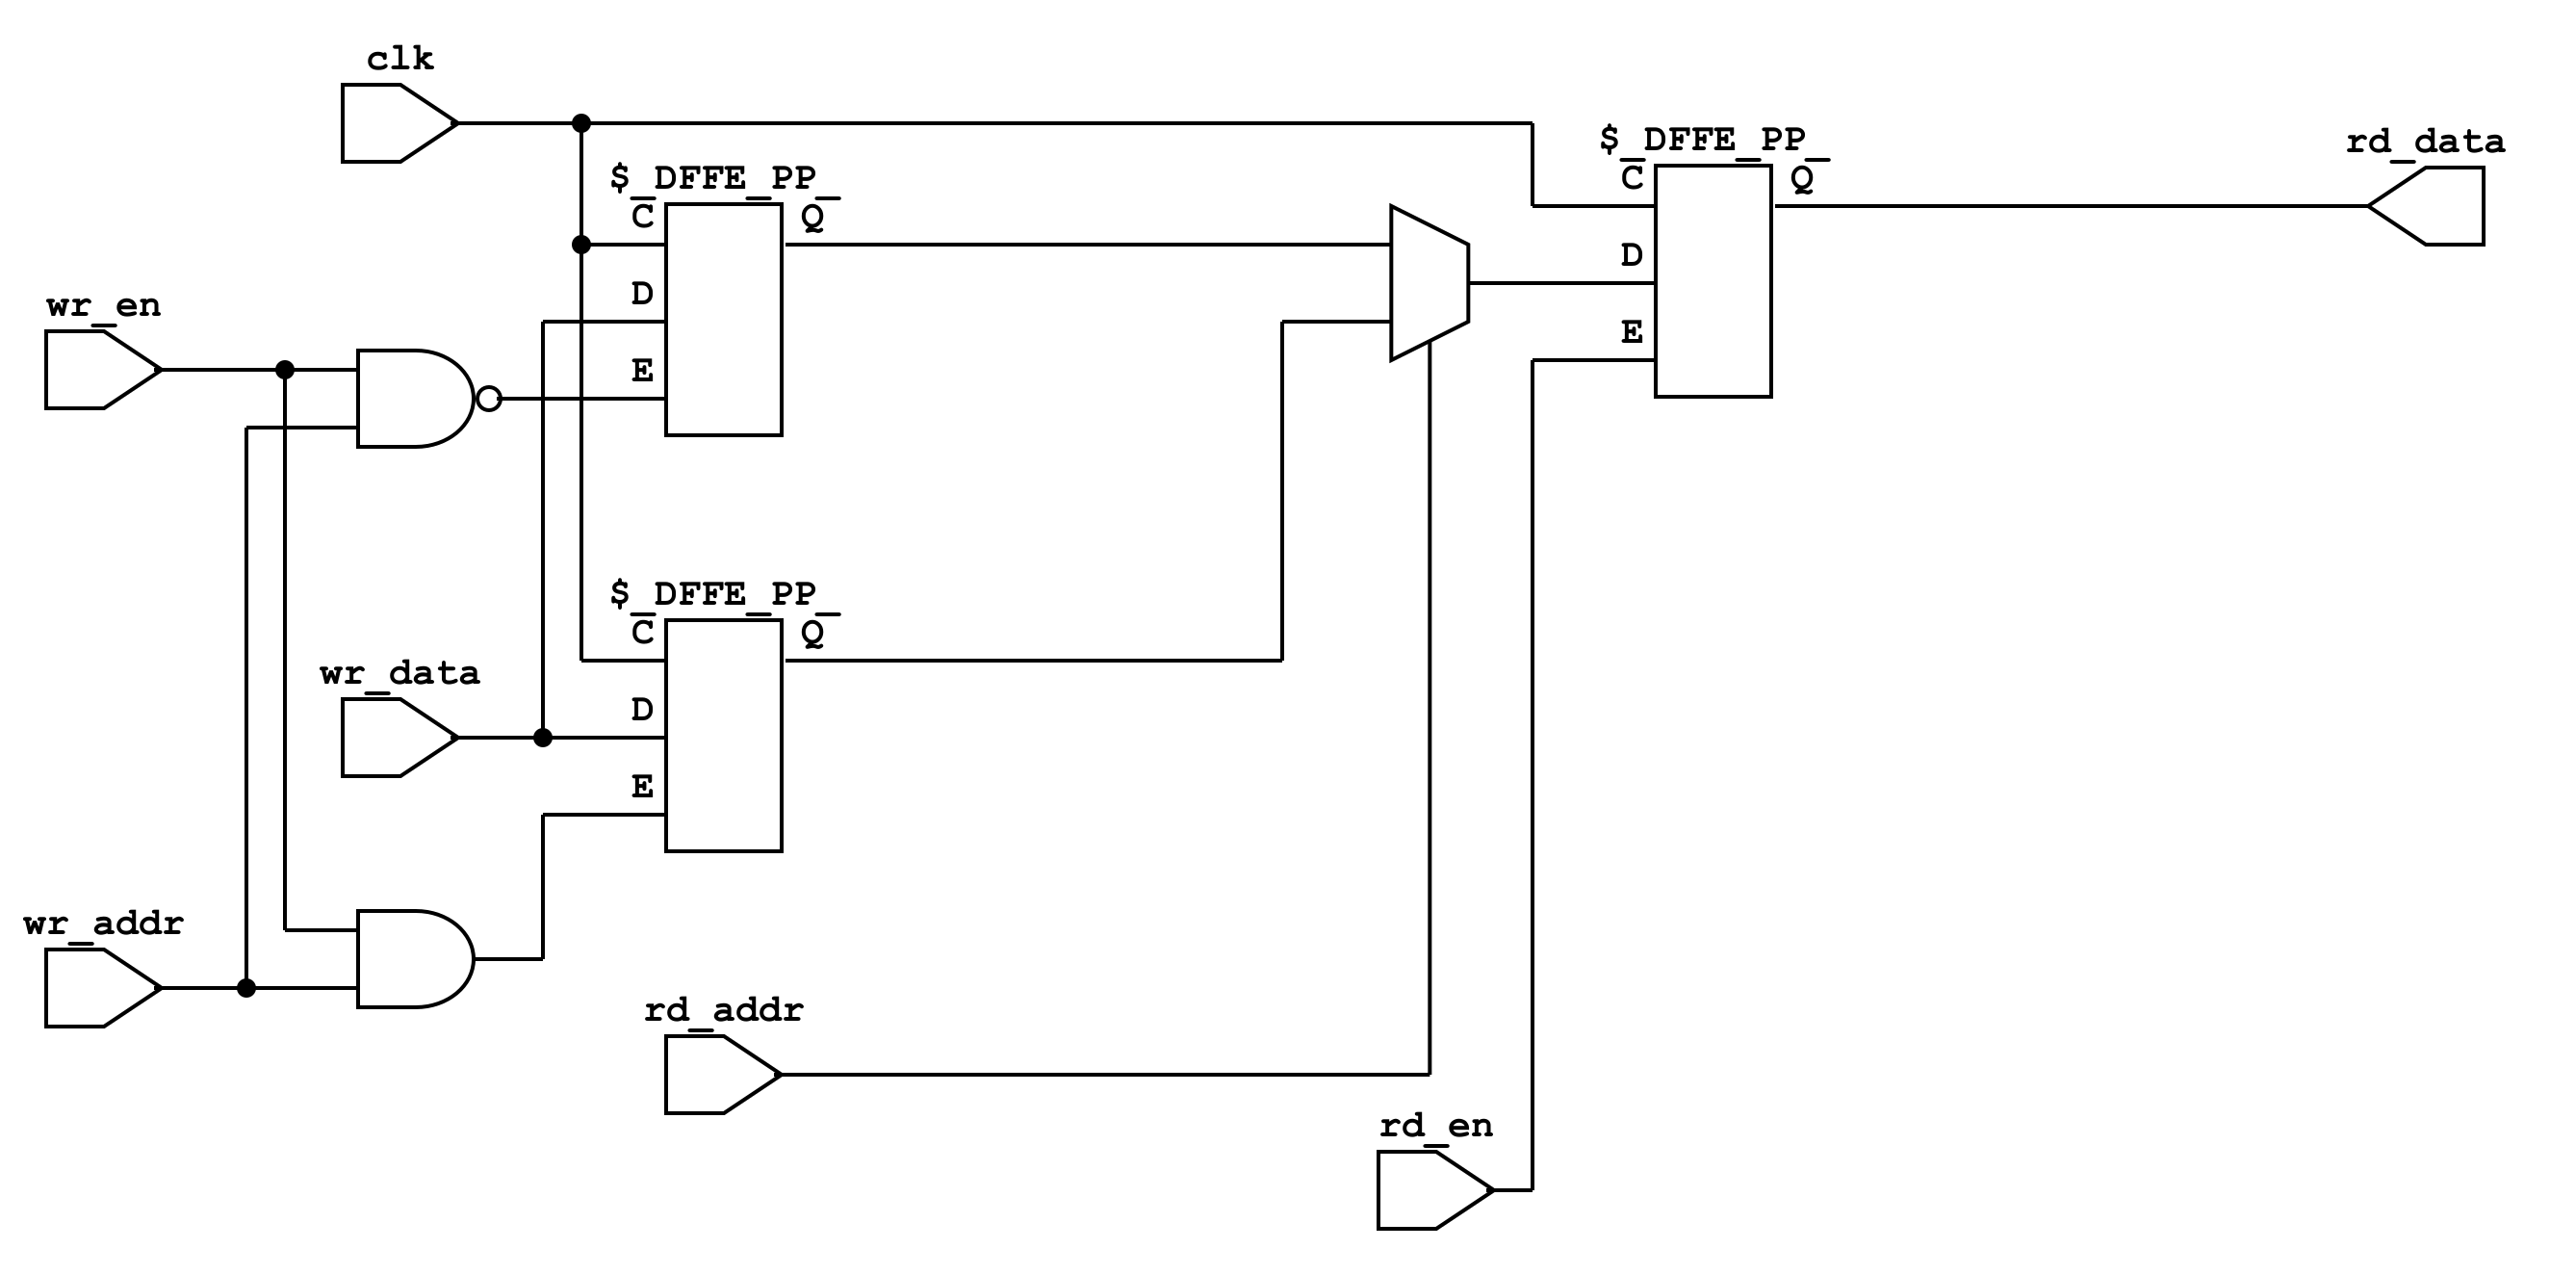
\includegraphics[width=.99\columnwidth]{sync_ram_2x1_gate.png}
\caption{Gate-level implementation of a two-word, one-bit synchronous RAM.
Two enabled flip-flops store the data; a multiplexer and output flip-flop
provide the registered read path.}
\label{fig:gateram}
\end{figure}

Generic gate counts characterize circuit structure. Physical area and
critical-path delay require technology mapping, SRAM macro selection, and
timing analysis.

\section{Verification and Experimental Setup}
\subsection{RTL Workload and Correctness Checks}
The RAM, MAC, and controller are Verilog-2001-style synthesizable RTL.
Only the testbench and experiment driver are simulation infrastructure.
Icarus Verilog 14.0 compiles each parameterization with \texttt{-g2005}.
For tile $t$ and element $i$, the deterministic input operands are
\begin{align}
a_{t,i}&=((t+i)\bmod 15)+1,\\
w_{t,i}&=((3t+2i)\bmod 15)+1.
\end{align}
The expected output is $y_t=\sum_{i=0}^{T-1}a_{t,i}w_{t,i}$. The testbench
checks both $y_t$ and tile ID at every completion, detects duplicates, and
asserts that the one loader and one MAC never occupy multiple banks. It also
checks legal bank allocation, bank-state accounting, and runtime mode
limits. The functional suite contains 14 parameterizations. The RH matrix
contains 129 configurations for which independent analysis verifies active
cycle sums, operation counts, and structural throughput bounds. Thirteen
reported metrics per configuration also agree with a frozen RH reference.
A phase-case VCD establishes the six observed bank-limit transitions.

Handoff correctness is checked across 84 stress configurations covering
single-bank reuse, non-power-of-two bank counts, minimum service targets,
one-tile workloads, larger tiles, and variable or phase-changing timing.
Issue scoreboards detect duplicate MAC acceptance, and bank assertions
reject ownership and read/write collisions. Acceptance-to-completion traces
verify each load and MAC service interval independently of the utilization
counters. All reported configurations pass their arithmetic,
protocol, and accounting checks.

\begin{table}[t]
\centering\caption{Simulation and trace-based verification results.}
\label{tab:verification}\scriptsize
\setlength{\tabcolsep}{3pt}
\begin{tabular}{p{.59\columnwidth}r}
\toprule
Check & Result\\
\midrule
Self-checking functional parameterizations & 14/14 pass\\
RH configurations with checked tile results & 129/129 pass\\
Independent cycle/operation checks & 129/129 pass\\
VCD mode transitions checked & 6\\
RH reference agreement: 13 metrics per case & 129/129\\
Handoff correctness stress configurations & 84/84 pass\\
\bottomrule
\end{tabular}
\end{table}

\subsection{Matched Experimental Matrix}
All policies receive identical tile values and the same deterministic
latency sequence in a matched scenario. There is one loader, one MAC,
eight-bit operands, and a four-pair tile in the principal comparisons.
Each bank has four addressable words unless stated otherwise. The transfer
target has a floor of $T$ clocks because the loader writes $T$ pairs. The
compute target has a floor of $T+2$ clocks for the synchronous read pipeline.
No clock frequency, DRAM channel timing, or physical SRAM macro is assumed.

\begin{table}[t]
\centering\caption{Experiment families and base transfer/compute targets
in clocks per tile. Tiles contain four operand pairs except in the
larger-tile family, which uses 16. Profiles are identical across policies.}
\label{tab:matrix}\scriptsize
\setlength{\tabcolsep}{3pt}
\begin{tabular}{p{.34\columnwidth}rrp{.30\columnwidth}}
\toprule
Family & Tiles & Base & Profile\\
\midrule
Fixed balanced & 32 & 8/8 & Constant\\
Fixed slower compute & 64 & 8/20 & Constant\\
Balanced adaptation & 64 & 8/8 & Constant\\
Fixed slower memory & 64 & 32/8 & Constant\\
Variable adaptation & 64 & 8/8 & Per-tile increments\\
Three-phase adaptation & 96 & 8/8 & Slow compute / irregular memory / slow compute\\
Minimum targets & 64 & 4/6 & Constant\\
Larger tile & 16 & 16/20 & Per-tile increments\\
One tile & 1 & 8/8 & Constant\\
Bank scaling & 32 & 8/8 & Variable; 2, 3, 4, 6, 8 banks\\
\bottomrule
\end{tabular}
\end{table}

Table~\ref{tab:matrix} summarizes the evaluated workload families. The broader
matrix also varies tile count, tile size, and memory-to-compute ratio.
The standard variable transfer increments repeat
$[0,8,0,7,18,0,4,13,2,10]$ by tile ID; compute increments repeat
$[0,4,0,8,2]$. In the 96-tile phase experiment, the outer thirds add
12 compute clocks per tile, while the middle third uses base compute
latency and transfer increments
$[0,16,0,10,22,1,4,19,0,12]$. These are deterministic stress profiles,
not recorded neural-network traces. The exact parameters and raw logs are
available in the project archive.

The primary comparison evaluates Fixed 4 and the proposed controller
across eight workload families with 1, 16, 64, or 96 tiles. Each matched
pair receives identical operands, service targets, and latency profiles.
Single-buffer and ping-pong baselines establish the benefit of overlapping
loading and computation. The 32-tile buffering and bank-count sweeps use
RH control to characterize storage capacity and allocation policy.

\section{Experimental Results}
\subsection{End-to-End Performance}
Table~\ref{tab:lookahead} compares the proposed controller with Fixed 4.
For the balanced 64-tile workload, the proposed design requires
522 cycles compared with 713 cycles for Fixed 4, a reduction of 26.79\%.
Both configurations perform 512 MAC-active and 512 load-active clocks;
MAC-idle time decreases from 201 to ten clocks.
The first tile finishes loading at edge 9, the last MAC finishes at edge
521, and its result is retired at edge 522. The active-cycle counts and
completion trace attribute the reduction to handoff overhead.

\begin{table*}[t]
\centering\caption{Execution cycles for Fixed 4 and the proposed controller
under identical per-tile service targets. Reduction is relative to Fixed 4;
the average allocation limit refers to the proposed controller.}
\label{tab:lookahead}\small
\setlength{\tabcolsep}{5pt}
\begin{tabular}{lrrrr}
\toprule
Workload & Fixed 4 & Proposed & Reduction & Avg. limit\\
\midrule
Compute-bound, 64 tiles & 1481 & 1290 & 12.90\% & 2.025\\
Balanced, 64 tiles & 713 & 522 & 26.79\% & 2.061\\
Memory-bound, 64 tiles & 2123 & 2058 & 3.06\% & 3.953\\
Variable, 64 tiles & 983 & 925 & 5.90\% & 3.069\\
Phase change, 96 tiles & 1991 & 1808 & 9.19\% & 2.619\\
Minimum targets, 64 tiles & 581 & 390 & 32.87\% & 2.000\\
Larger tile, 16 tiles & 429 & 403 & 6.06\% & 2.079\\
One tile & 20 & 18 & 10.00\% & 2.000\\
\bottomrule
\end{tabular}
\end{table*}

\begin{figure*}[t]
\centering
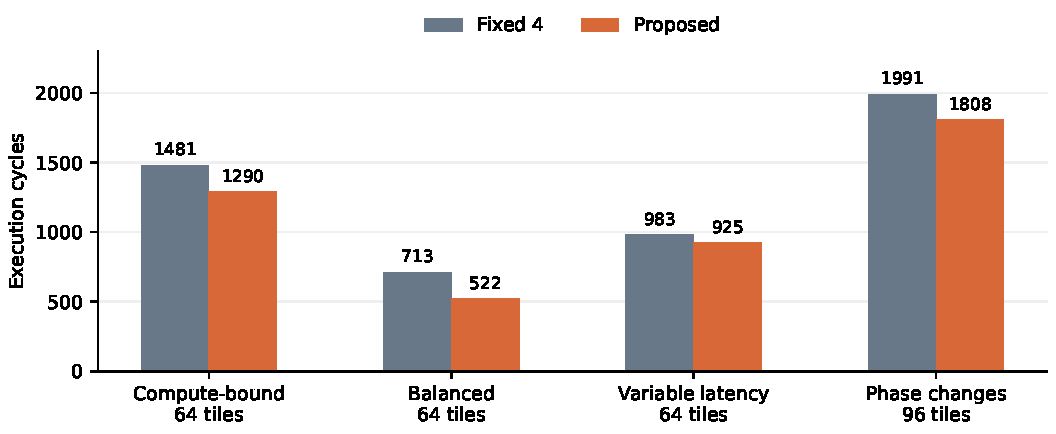
\includegraphics[width=.94\textwidth]{paper_primary_cycles.pdf}
\caption{End-to-end execution cycles for Fixed 4 and the proposed
controller across the four principal workloads.}
\label{fig:lookaheadcycles}
\end{figure*}

Under variable latency, the proposed controller requires 925 cycles
compared with 983 for Fixed 4, a 5.90\% reduction, at an average allocation
limit of 3.069. In the phase workload, it requires 1808 cycles compared
with 1991 for Fixed 4, a 9.19\% reduction, at an average limit of 2.619.
The complete controller therefore improves execution time while reducing
average allocation eligibility across these workloads.

\subsection{Fixed and Variable Buffering}
The buffering experiments use RH control to isolate bank capacity and
allocation policy. At constant 8/8 latency, ping-pong reduces 32-tile
execution from 640 to 361 cycles (1.773$\times$ versus single), but four
banks offer no further improvement. With the deterministic variable profile,
ping-pong takes 539 and fixed four-bank takes 497 cycles, a 1.0845$\times$
speedup over ping-pong. Its compute-idle count falls from 195 to 153 clocks.
The same fixed-four result appears with static cyclic mapping, so this
specific gain reflects additional independent tile slots rather than a
measured benefit from dynamic arbitration at equal bank count.

\begin{table}[t]
\centering\caption{Execution cycles with RH control, 32 tiles, four pairs
per tile, and base transfer/compute targets of 8/8.}
\label{tab:basic}\scriptsize
\setlength{\tabcolsep}{3pt}
\begin{tabular}{lrrrr}
\toprule
Latency & Single & Ping-pong & Avail. 4 & Cyclic 4\\
\midrule
Fixed & 640 & 361 & 361 & 361\\
Variable & 922 & 539 & 497 & 497\\
\bottomrule
\end{tabular}
\end{table}

The bank-count sweep in Fig.~\ref{fig:scaling} for variable base 8/8 gives
539 cycles at two banks,
497 at three, and 497 at four, six, and eight. Thus the first additional
slot matters for this pattern, while further slots saturate. This is not a
general optimum bank count: there is still one transfer interface and one
MAC, and the latency sequences are specific to the synthetic workload.

\begin{figure}[t]
\centering
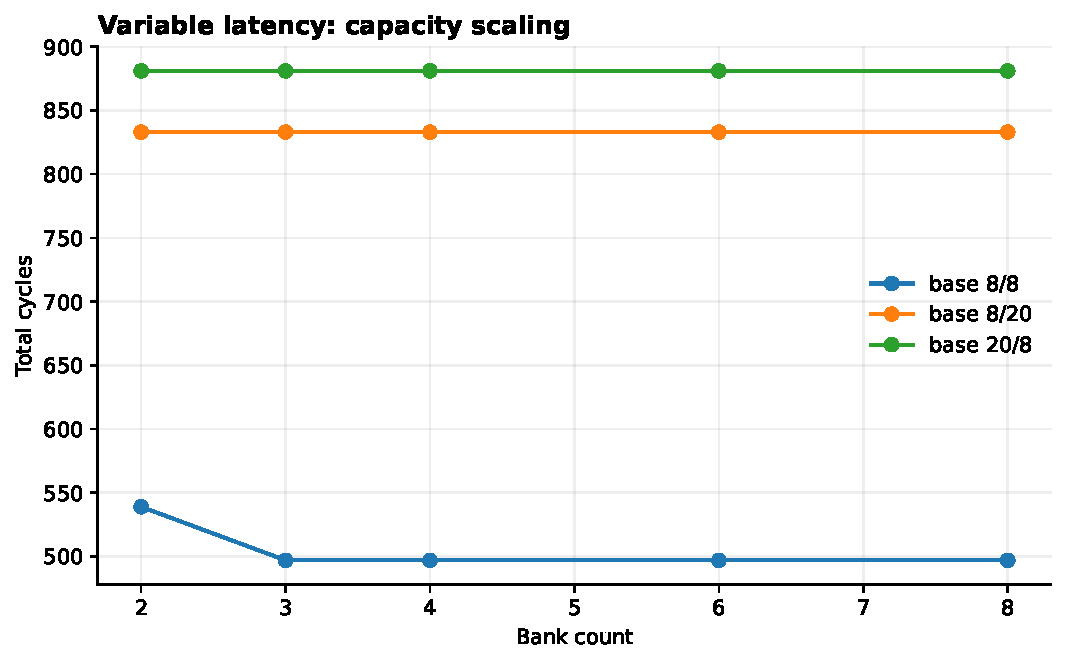
\includegraphics[width=\columnwidth]{bank_scaling_cycles.pdf}
\caption{Bank-count sweep under the deterministic variable profile. Only
the base 8/8 case benefits from moving from two to three banks in this
sweep; additional banks do not reduce measured cycles.}
\label{fig:scaling}
\end{figure}

\begin{table}[t]
\centering\caption{Baseline and proposed configurations for 64 tiles.
Idle denotes MAC-idle clocks; $\bar B$ is the average allocation limit.}
\label{tab:runtime}\scriptsize
\begin{tabular}{lrrrr}
\toprule
Configuration & Cycles & Idle & Util. (\%) & $\bar B$\\
\midrule
\multicolumn{5}{l}{\textit{Compute-bound}}\\
Ping-pong & 1481 & 201 & 86.43 & 2.000\\
Fixed 4 & 1481 & 201 & 86.43 & 4.000\\
\textbf{Proposed} & \textbf{1290} & \textbf{10} & \textbf{99.22} & \textbf{2.025}\\
\midrule
\multicolumn{5}{l}{\textit{Balanced}}\\
Ping-pong & 713 & 201 & 71.81 & 2.000\\
Fixed 4 & 713 & 201 & 71.81 & 4.000\\
\textbf{Proposed} & \textbf{522} & \textbf{10} & \textbf{98.08} & \textbf{2.061}\\
\midrule
\multicolumn{5}{l}{\textit{Variable latency}}\\
Ping-pong & 1072 & 380 & 64.55 & 2.000\\
Fixed 4 & 983 & 291 & 70.40 & 4.000\\
\textbf{Proposed} & \textbf{925} & \textbf{233} & \textbf{74.81} & \textbf{3.069}\\
\bottomrule
\end{tabular}
\end{table}

\subsection{Runtime Adaptation and Phase Changes}
Table~\ref{tab:runtime} compares the proposed controller with ping-pong
and Fixed 4. In the stable workloads, the proposed design averages
2.025 and 2.061 eligible banks and reduces idle time from 201 to ten
clocks. Under variable latency, it requires 925 cycles at 74.81\%
utilization, compared with 983 cycles at 70.40\% for Fixed 4.

For the 96-tile phase workload, the proposed controller requires 1808
cycles compared with 1991 for Fixed 4 (Table~\ref{tab:phase}). Its 272
MAC-idle clocks are 183 fewer than Fixed 4's 455. All configurations perform
1536 MAC-active clocks, so the cycle difference corresponds directly to
recovered overlap.

\begin{table}[t]
\centering\caption{Baseline and proposed configurations for the 96-tile
phase workload. All perform 1536 MAC-active clocks and 384 MAC operations.}
\label{tab:phase}\scriptsize
\setlength{\tabcolsep}{3pt}
\begin{tabular}{lrrrr}
\toprule
Configuration & Cycles & Idle & Util. (\%) & $\bar B$\\
\midrule
Single & 2950 & 1414 & 52.07 & 1.000\\
Ping-pong & 2054 & 518 & 74.78 & 2.000\\
Fixed 4 & 1991 & 455 & 77.15 & 4.000\\
\textbf{Proposed} & \textbf{1808} & \textbf{272} & \textbf{84.96} & \textbf{2.619}\\
\bottomrule
\end{tabular}
\end{table}

The proposed controller's trajectory in Fig.~\ref{fig:trace} starts at two eligible banks,
briefly reaches three at execution cycle 32, and returns to two at 64.
It rises to three at 672 and four at 704 as transfer latency becomes
irregular, then falls to three at 1216 and two at 1248. Mode occupancy is
1200 clocks at limit two, 96 at three, and 512 at four, totaling 1808
clocks and an average limit of 2.619. The initial excursion indicates
sensitivity of the starvation threshold to pipeline fill.

\begin{figure}[t]
\centering
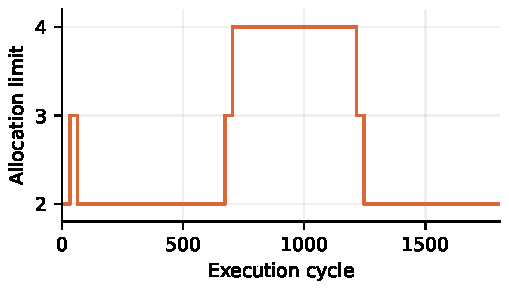
\includegraphics[width=\columnwidth]{paper_proposed_phase_trace.pdf}
\caption{Runtime bank eligibility during the three-phase workload under
the proposed controller.}
\label{fig:trace}
\end{figure}

\subsection{Equal Storage Capacity}
Two eight-word banks and four four-word banks each instantiate 16 RAM words.
Table~\ref{tab:storage} reports the variable and phase workloads at this
storage capacity. Their cycle counts match those in the
four-word-per-bank experiments because each bank holds at most one tile,
irrespective of its addressable depth. Equal word count therefore does not
imply equal independent tile capacity or decoder structure.

\begin{table}[t]
\centering\caption{Execution cycles at equal storage capacity:
two eight-word banks or four four-word banks, with four pairs per tile.}
\label{tab:storage}\scriptsize
\setlength{\tabcolsep}{2pt}
\begin{tabular}{lrrr}
\toprule
Case & Ping-pong & Fixed 4 & Proposed\\
\midrule
Variable, 64 tiles & 1072 & 983 & 925\\
Phase, 96 tiles & 2054 & 1991 & 1808\\
\bottomrule
\end{tabular}
\end{table}

\section{Discussion, Limitations, and Future Work}
\subsection{Buffer Capacity and Handoff Overhead}
The buffering results distinguish overlap from capacity. Two-bank
ping-pong overlaps loading and computation, while a third independent tile
slot absorbs the transfer bursts in the variable 8/8 workload. At four
banks, availability and static cyclic scheduling produce identical cycle
counts in the matched RH experiments. The observed improvement over
ping-pong is therefore attributable to independent tile capacity within
the evaluated sequential tile stream.

The proposed design addresses control overhead and bank eligibility
together. Completion-aware issue removes idle handoff clocks, while the
allocation limit adapts to observed compute starvation. During the phase
workload, eligibility increases to four banks and subsequently returns to
two. The initial two-to-three excursion indicates sensitivity to pipeline
fill, and the observation window introduces a finite response delay.
Despite this delay, the complete controller reduces execution cycles
relative to Fixed 4 under every workload in Table~\ref{tab:lookahead}.

\subsection{Model Scope and Limitations}
The RAM model is behavioral RTL rather than a characterized SRAM macro. Four
physical banks remain present even when the limit is two, so the experiment
does not establish dynamic or leakage power savings, nor an area reduction.
The model omits a DRAM protocol, a full CNN dataflow, cache hierarchy,
physical timing, placement, and clock-frequency effects. A single loader
also caps memory-bound throughput independently of bank count. The
synthetic, deterministic latency profiles are useful controlled stresses
but do not represent a measured application distribution. Bank depth and
tile-slot count are entangled in the equal-word experiment.

Cycle reduction assumes the same clock period. The look-ahead arbiter adds
a completion-to-issue combinational path, so placement and timing are
needed to establish an elapsed-time improvement. Generic synthesis cell
counts provide a structural check, not a physical cost measurement.
The comparison evaluates the combined controller against the specified
Fixed 4 implementation. It does not establish that restricting bank
eligibility alone reduces execution cycles.

Future evaluation will require application layer traces, sensitivity
analysis of observation windows and thresholds, and characterization of
startup adaptation. Multiple transfer channels would test the policy beyond
the single-loader throughput limit. Technology mapping, SRAM macro
integration, timing closure, and energy measurements are required to
assess the physical cost of eligibility control and completion-aware issue.

\section{Conclusion}
Completion-aware handoffs reduce scratchpad execution cycles with
the same four physical banks, one loader, one MAC, and unchanged tile
service times. Combined with runtime eligibility, they reduce cycles by
26.79\% in the balanced case, 5.90\% under variable latency, and 9.19\% under
phase changes relative to Fixed 4. The corresponding average allocation
limits are 2.061, 3.069, and 2.619 banks. These results characterize the
complete proposed controller, which combines completion-aware handoffs
with runtime bank eligibility. Physical timing and energy characterization
remain necessary to evaluate implementation efficiency.

\section{Artifact Availability}
The reproducibility package comprises parameterized Verilog RTL, a
self-checking testbench, deterministic workload generators, simulator
logs, CSV summaries, VCD traces, and logic-synthesis scripts. Each
performance record is accepted only after arithmetic and protocol checks
pass. The evaluation dataset includes per-tile acceptance and completion
events, configuration parameters, and source hashes. Plotting scripts
derive the reported figures directly from these records. The package
README specifies tool setup and commands for simulation, independent
analysis, synthesis, and figure generation.

\begin{thebibliography}{4}
\bibitem{sze2017survey} V. Sze, Y.-H. Chen, T.-J. Yang, and J. S. Emer,
``Efficient Processing of Deep Neural Networks: A Tutorial and Survey,''
\emph{Proc. IEEE}, vol. 105, no. 12, pp. 2295--2329, 2017,
doi: 10.1109/JPROC.2017.2761740.
\bibitem{chen2017eyeriss} Y.-H. Chen, T. Krishna, J. S. Emer, and V. Sze,
``Eyeriss: An Energy-Efficient Reconfigurable Accelerator for Deep
Convolutional Neural Networks,'' \emph{IEEE J. Solid-State Circuits}, 2017,
doi: 10.1109/JSSC.2016.2616357.
\bibitem{jouppi2017tpu} N. P. Jouppi \emph{et al.},
``In-Datacenter Performance Analysis of a Tensor Processing Unit,''
\emph{Proc. ISCA}, 2017, doi: 10.1145/3079856.3080246.
\bibitem{chen2019eyerissv2} Y.-H. Chen, T.-J. Yang, J. S. Emer, and V. Sze,
``Eyeriss v2: A Flexible Accelerator for Emerging Deep Neural Networks on
Mobile Devices,'' \emph{IEEE J. Emerging Sel. Topics Circuits Syst.},
vol. 9, no. 2, pp. 292--308, 2019, doi: 10.1109/JETCAS.2019.2910232.
\end{thebibliography}
\end{document}
